\documentclass[10pt,letterpaper]{article}
\usepackage[margin=0.68in]{geometry}
\usepackage{graphicx}
\usepackage{booktabs}
\usepackage{tabularx}
\usepackage{array}
\usepackage{fancyhdr}
\usepackage[colorlinks=true,linkcolor=blue,urlcolor=blue]{hyperref}
\setlength{\headheight}{24pt}
\setlength{\parskip}{3pt}
\setlength{\parindent}{0pt}
\pagestyle{fancy}
\fancyhf{}
\lhead{Finite-GMC 40-$M_\odot$ bubble}
\rhead{20 October 2026, 16:00 EDT}
\cfoot{\thepage}

\begin{document}
\title{A Wolf--Rayet Bubble in a Finite Cloud\\Primer and Controlled Shell-Resolution Test}
\author{GRB model-fitting meeting book}
\date{20 October 2026, 16:00 EDT\\Premeeting evidence edition; checked 15:11 EDT}
\maketitle

\begin{abstract}
The short direct-Wolf--Rayet (WR) experiment produces a strong numerical swept shell in the $n_{\rm ref}=20{,}000\,{\rm cm}^{-3}$ finite-GMC cases. At 0.0015 Myr, the matched 16,384-cell, inward-refined, 2.5-pc-domain calculations place the inner 10\% rise at 0.063717 and 0.063751 pc for GMC background densities 1,000 and 2,000 $\mathrm{cm}^{-3}$. Their 10--90\% rises span 5.38 and 5.56 native cells. The independently validated 20,480-cell GMC 1,000 wind places the same rise at 0.064087 pc and 5.58 cells; its physical rise width still changes. The GMC 2,000 20,480-cell atmosphere passed, but the matching wind is held because its host-measured runtime projection fails the required guard margin. These results do not establish a converged or physical shell width. No swept shell has been identified with a WR termination shock or a GRB fit.
\end{abstract}

\section{Primer: The Star, the Cloud, and the Clock}
A giant molecular cloud (GMC) is a large reservoir of cold gas. Gravity can gather some of that gas into a denser core, from which a massive star forms. Once the star shines, its ultraviolet photons ionize nearby hydrogen (an H\,II region), while its stellar wind carries mass, momentum, and energy outward. These forms of feedback can excavate or disperse the natal gas. Consequently, a star entering its final WR phase need not still sit inside the undisturbed cloud in which it formed. That uncertain earlier history is the central physical caveat of our calculation.

\textbf{Scale guide.} One parsec (pc) is 3.26 light-years. $\dot M$ is the mass expelled each year, measured in solar masses ($M_\odot$) per year; wind speed is in km s$^{-1}$. $n_{\rm H}$ counts hydrogen nuclei per cm$^3$. ``Subparsec'' describes a size, not which of several wind or cloud boundaries has been measured.

\section{Which Winds Could Precede the Burst?}
An illustrative path is a hot, hydrogen-burning main-sequence (MS) star, a cool and swollen red supergiant (RSG), then a hot WR star stripped of much of its outer hydrogen. It is \emph{not} a required path for every initially $40\,M_\odot$ star: mass loss, metallicity, rotation, and binary interaction matter. Spectroscopic work suggests an RSG history for many WN stars in the 20--40-$M_\odot$ initial-mass range, but the evolutionary route remains model-dependent.

\begingroup\small\renewcommand{\arraystretch}{1.08}\setlength{\tabcolsep}{5pt}
\begin{tabularx}{\textwidth}{@{}p{0.09\textwidth}>{\raggedright\arraybackslash}X p{0.27\textwidth}@{}}
\toprule
Stage & Illustrative wind and its effect & Value in source code \\
\midrule
MS & Hot star: strong UV and a fast wind can leave an H\,II region and a large older cavity. & $10^{-6}\,M_\odot\,{\rm yr}^{-1}$; 2,000 km s$^{-1}$ \\
RSG & Quiescent $\dot M\sim10^{-7}$--$10^{-5}\,M_\odot\,{\rm yr}^{-1}$; dusty or brief enhanced loss can approach $10^{-4}$. The slow, 10--30 km s$^{-1}$ wind deposits dense gas. & $5\times10^{-5}\,M_\odot\,{\rm yr}^{-1}$; 15 km s$^{-1}$ \\
WR & WN samples span roughly $2\times10^{-6}$--$3\times10^{-5}\,M_\odot\,{\rm yr}^{-1}$; fast winds commonly reach order 1,000--3,000 km s$^{-1}$. Subtype and metallicity matter. & $10^{-5}\,M_\odot\,{\rm yr}^{-1}$; 2,000 km s$^{-1}$ \\
\bottomrule
\end{tabularx}
\endgroup

The ranges describe different observed populations and modes of mass loss, not a prior for this particular star. RSG rates are especially uncertain; a brief high-loss episode should not be confused with a sustained quiescent wind. The present \emph{wind run skips the MS and RSG evolution entirely}: the source code contains these branches, but a 4.5-Myr phase offset selects WR conditions at the first time step. See \href{https://arxiv.org/abs/2001.07222}{Beasor et al. (2020)}, \href{https://arxiv.org/abs/1508.07003}{Mackey et al. (2015)}, \href{https://arxiv.org/abs/1401.5474}{Hainich et al. (2014)}, and \href{https://arxiv.org/abs/1201.6354}{Sander et al. (2012)}.

\clearpage
\section{Why a Subparsec WR Region Is Difficult}
For a steady freely expanding wind, $\rho_{\rm w}(r)=\dot M/(4\pi r^2v_{\rm w})$: its density falls as $r^{-2}$. Some GRB afterglows are instead modeled with a flatter surrounding density. One possibility is that the relativistic outflow has already crossed the \emph{wind termination shock} into shocked wind. A powerful WR wind usually places that transition too far from the star for this explanation to be easy. A smaller transition requires unusually strong local confinement, a weaker wind, or another restricted circumstance such as stellar motion or a binary companion; no one mechanism solves the problem generically \href{https://arxiv.org/abs/astro-ph/0605698}{(van Marle et al. 2006)}.

\begingroup\small\renewcommand{\arraystretch}{1.08}
\begin{tabularx}{\textwidth}{@{}p{0.28\textwidth}>{\raggedright\arraybackslash}X@{}}
\toprule
Moving outward from the star & What the boundary means \\
\midrule
Free WR wind $\rightarrow$ termination shock & The $r^{-2}$ wind first slows strongly; this is the transition relevant to the wind-like versus shocked-wind afterglow question. \\
Shocked wind $\rightarrow$ swept shell & The WR-driven flow pushes up a density enhancement in older wind or ambient gas. Our measured $R_{10}$ is the inner 10\% rise of this \emph{swept density excess}, not the termination-shock radius. \\
Ambient cloud $\rightarrow$ GMC edge & The cloud outside the shell can resist its expansion. The modeled GMC edge at 15 pc is beyond the evolved 2.5-pc mesh but enters the 20-pc pressure construction; it is not either wind boundary. \\
\bottomrule
\end{tabularx}
\endgroup

The simple ram-pressure scale is
\[
 P_{\rm ram}(r)=\frac{\dot M_{\rm WR}v_{\rm WR}}{4\pi r^2},\qquad
 R_{\rm t}\sim\left(\frac{\dot M_{\rm WR}v_{\rm WR}}{4\pi P_{\rm conf}}\right)^{1/2}.
\]
Here $P_{\rm conf}$ is the pressure actually encountered by the free wind, generally mediated by shocked gas; it is not determined by cloud number density alone. With our adopted WR wind, a termination shock at 0.1 pc would require a characteristic pressure of about $10^{-7}$ dyn cm$^{-2}$ in this idealized balance. A cold dense cloud may have large mass and column density yet modest thermal pressure. Gravity, turbulence, ionization, wind history, and local shell structure therefore matter as much as the label ``dense cloud.''

\section{What Our Numerical Experiment Does and Does Not Test}
We prescribe a spherical finite cloud: $n_{\rm ref}=20{,}000$ cm$^{-3}$ normalizes the core profile at 1 pc before its edge taper; it is not a central density. The flattened inner scale is 0.2 pc, the core extends to about 2 pc, and the GMC background is 1,000 or 2,000 cm$^{-3}$ before tapering toward 10 cm$^{-3}$ outside a 15-pc GMC. The gas starts at rest in a hydrostatic pressure profile built from the star plus enclosed cloud mass, anchored at 20 pc. The mesh evolves only 0.0002--2.5 pc, the region where the early shell lies.

The 0.1-Myr \emph{static control} has neither wind nor ionization: it tests whether that prescribed atmosphere stays stable. The separate \emph{wind run} switches on the WR wind and a simplified ionizing-photon treatment for just 0.0015 Myr (1,500 years). Gravity follows the initial mass profile and is held fixed; an effective 0.72-km-s$^{-1}$ support term is prescribed. Radiative cooling and thermal conduction are off. The model is one-dimensional: it cannot form clumps, holes, turbulence, or asymmetric escape paths.

If the natal dense gas survives earlier feedback, this setup can produce a compact \emph{early swept shell} embedded within the modeled core and GMC. That is the conditional sense in which we expect containment. It does not prove the cloud remains cold throughout the ionized inner region, that a real star retains its natal cloud until WR, that the shell stays subparsec over the WR lifetime, or that the termination shock is subparsec. An MS/RSG-preconditioned cloud and the missing cooling/geometry physics are separate tests, not adjustments silently folded into this result.

\clearpage
\section{What We Can Say Now}
\begin{itemize}
\item The finite-GMC initial states, two 16,384-cell WR winds, and the new 20,480-cell GMC 1,000 WR wind passed independent exact-age, output-count, finite-positive, outer-state, wind-speed, and mass-flux checks. The current run is a \emph{direct WR wind into an initial cloud}, not a full main-sequence/RSG/WR evolutionary bubble.
\item The matched GMC 1,000/2,000 cases have nearly the same shell radius at 0.0015 Myr. Both meet the numerical shell gate and have at least five cells across the local 10--90\% rise. The physical rise width and radius still move with mesh grading.
\item Quality-gated shell-radius coverage is 13 of 20 logarithmic bins from 0.001 to 10 pc; no accepted case lies below 0.0251 pc. Selected negative-$k$ GRB radii, 0.001225--0.719437 pc, are analytic, model-dependent first-to-last sampled radii, not measured shell locations.
\end{itemize}

\section{Model and Numerical Gates}
\begingroup\small\renewcommand{\arraystretch}{1.08}
\begin{tabularx}{\textwidth}{@{}p{0.27\textwidth}>{\raggedright\arraybackslash}X@{}}
\toprule
Item & Fixed setup or acceptance rule \\
\midrule
Star and cloud & $40\,M_\odot$; $n_{\rm ref}=20{,}000\,{\rm cm}^{-3}$; GMC backgrounds 1,000 and 2,000 $\mathrm{cm}^{-3}$; finite 15-pc GMC, 2-pc core, 0.5-pc core edge. \\
Hydrodynamics & Spherical 1D; fixed cloud gravity and 0.72 km s$^{-1}$ support; radiative cooling and thermal conduction disabled. \\
WR shortcut & $v_{\rm WR}\simeq 2000$ km s$^{-1}$ and $\dot M_{\rm WR}\simeq10^{-5}\,M_\odot\,{\rm yr}^{-1}$, applied directly at the start of a 0.0015-Myr wind stage. \\
Matched domain & Inner boundary 0.0002 pc; evolved outer boundary 2.5 pc; hydrostatic atmosphere pressure anchor 20 pc. \\
Static gate & Guard exit 0; one normal AMRVAC finish; empty stderr; two VTUs; exact 0.1-Myr age; adequate cells across the \emph{calculated potential} ionization radius; finite positive initial mass, pressure, density and stable outer state. Ionization is off in this control. \\
Wind/shell gates & Seven VTUs and exact 0.0015-Myr endpoint; WR speed/flux; then H II $\geq10$, shell FWHM $\geq5$ native cells, contrast $\geq3$, FWHM/radius $\leq0.25$. Separately, local inner 10--90\% ramp $\geq5$ cells. \\
\bottomrule
\end{tabularx}
\endgroup

\section{Reading the Shell Plots}
The two panels on each following figure answer different questions. The full-radius panel shows the density profile from the star, through its broad inner precursor, to the shell; the dotted curve is the starting atmosphere. The zoom panel shows how sharply the density excess rises on the shell's \emph{inner} side. The vertical markers locate 10\%, 50\%, and 90\% of that rise. $R_{10}$ is its first measured radius, not the radius where free WR wind terminates.

We also report the shell's full width at half maximum (FWHM), peak-to-background contrast, and the 10--90\% inner rise in both parsecs and \emph{native cells}. A steep rise represented by only a few cells can look convincing on a plot while remaining grid-dependent. Our shell gate requires FWHM at least five cells and adequate contrast; the separate five-cell inner-rise criterion asks a stricter local-resolution question. Neither threshold proves a physical shock thickness. The clean comparison holds physics and saved age fixed while changing the mesh, and checks whether radii and widths settle in physical units.

\clearpage
\section{Matched-Age Shell Evidence}
\begingroup\small\renewcommand{\arraystretch}{1.08}\setlength{\tabcolsep}{4pt}
\begin{tabularx}{\textwidth}{@{}lrrrrrr@{}}
\toprule
GMC & First cell & $R_{10}$ & FWHM & Contrast & Rise & Rise \\
($\mathrm{cm}^{-3}$) & ($10^{-5}$ pc) & (pc) & (cells) & & (cells) & ($10^{-4}$ pc) \\
\midrule
1,000, 16,384 coarse & 2.50 & 0.062354 & 12.04 & 51.55 & 4.74 & 1.72 \\
1,000, 16,384 fine & 1.25 & 0.063717 & 15.55 & 54.09 & 5.38 & 1.48 \\
1,000, 20,480 fine & 1.25 & 0.064087 & 17.66 & 55.93 & 5.58 & 1.32 \\
2,000, 16,384 coarse & 2.50 & 0.062403 & 12.82 & 48.65 & 4.82 & 1.74 \\
2,000, 16,384 fine & 1.25 & 0.063751 & 16.47 & 51.21 & 5.56 & 1.53 \\
\bottomrule
\end{tabularx}
\endgroup

All rows are at 0.0015 Myr with the same inner/outer boundaries and physical parameters. The 16,384-cell fine rows halve only the first radial cell and change the geometric stretch ratio relative to their coarse controls; they do not double cell count. Relative to the matched 16,384-cell GMC 1,000 fine run, the new 20,480-cell rung shifts $R_{10}$ outward by 0.000369 pc (0.58\%) while the physical 10--90\% rise narrows from $1.48$ to $1.32\times10^{-4}$ pc. Thus the five-cell test is a \emph{numerical adequacy check}, not a convergence proof. The new wind validator found 1,173 initially ionized elements, $v_{\max}\simeq2000.8$ km s$^{-1}$, and $\dot M\simeq1.0002\times10^{-5}\,M_\odot\,{\rm yr}^{-1}$.

\begin{figure}[htbp]\centering
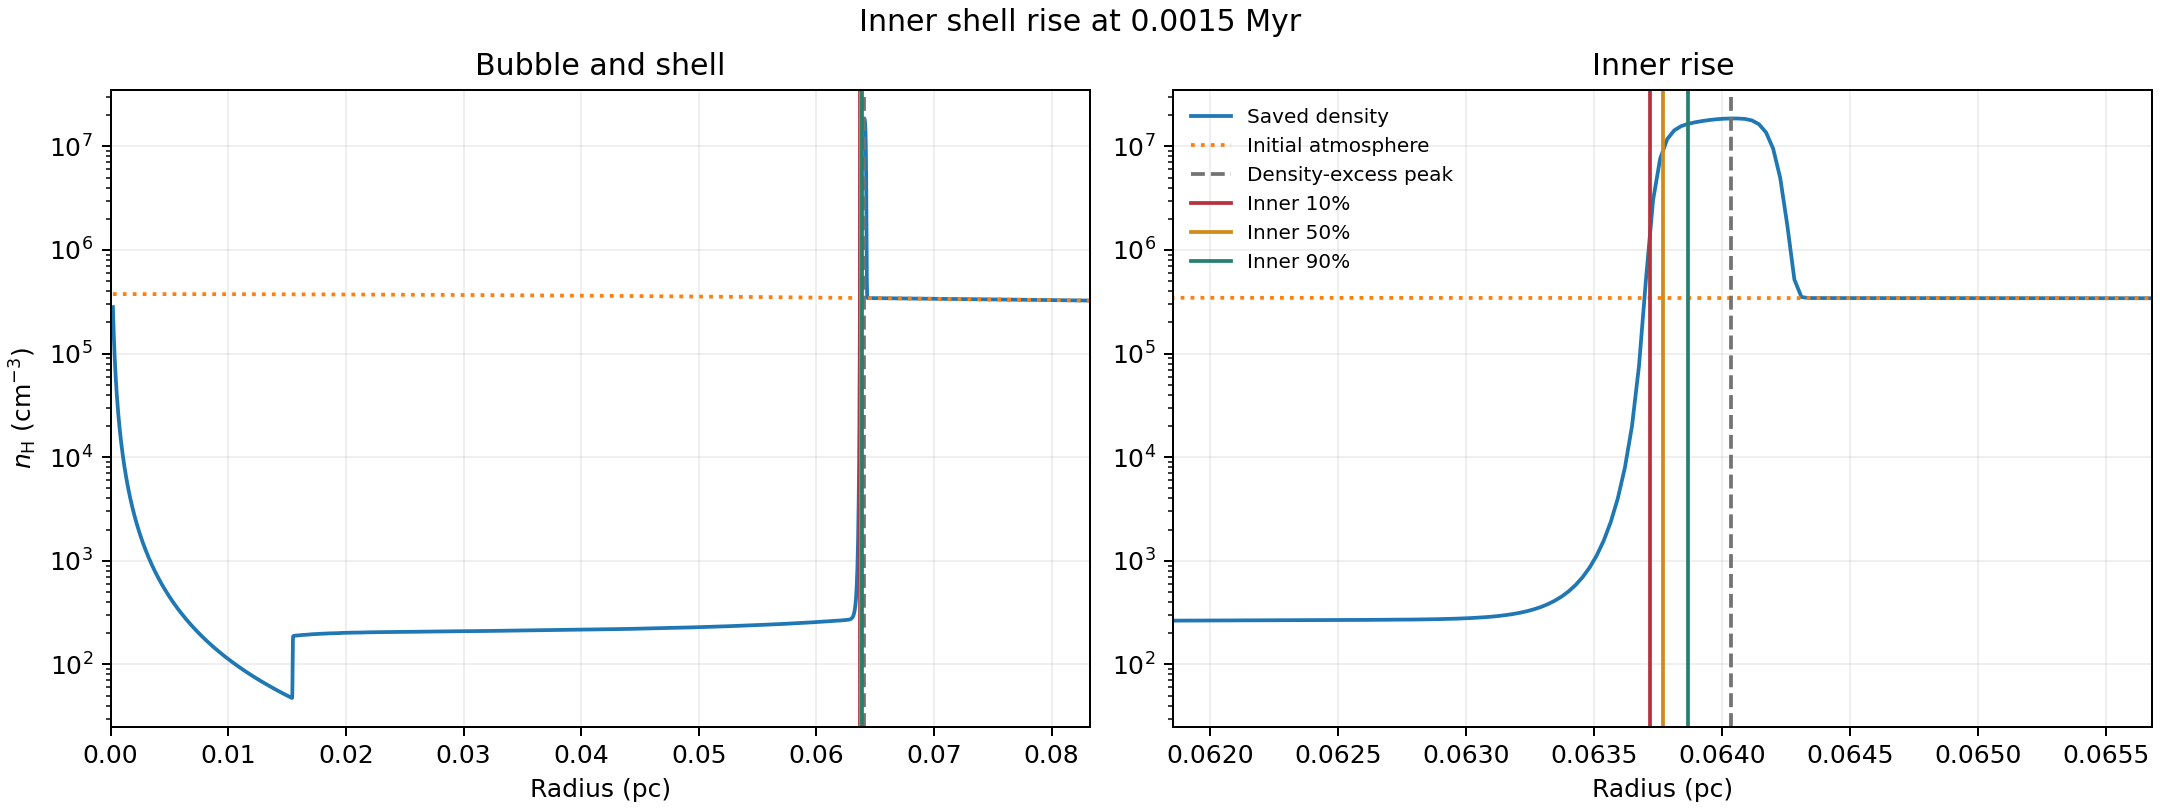
\includegraphics[width=0.98\textwidth,height=0.48\textheight,keepaspectratio]{images/gmc1000_inner_16384.png}
\caption{Validated GMC 1,000 fine-control profile at 0.0015 Myr. Left: the whole inward precursor through the shell, with the initial atmosphere dotted. Right: local inner 10/50/90\% rise and density-excess peak. The plotted width is a mesh-dependent numerical rise, not a physical shock thickness.}
\end{figure}

\clearpage
\section{Second Cloud-Mass Bracket}
\begin{figure}[htbp]\centering
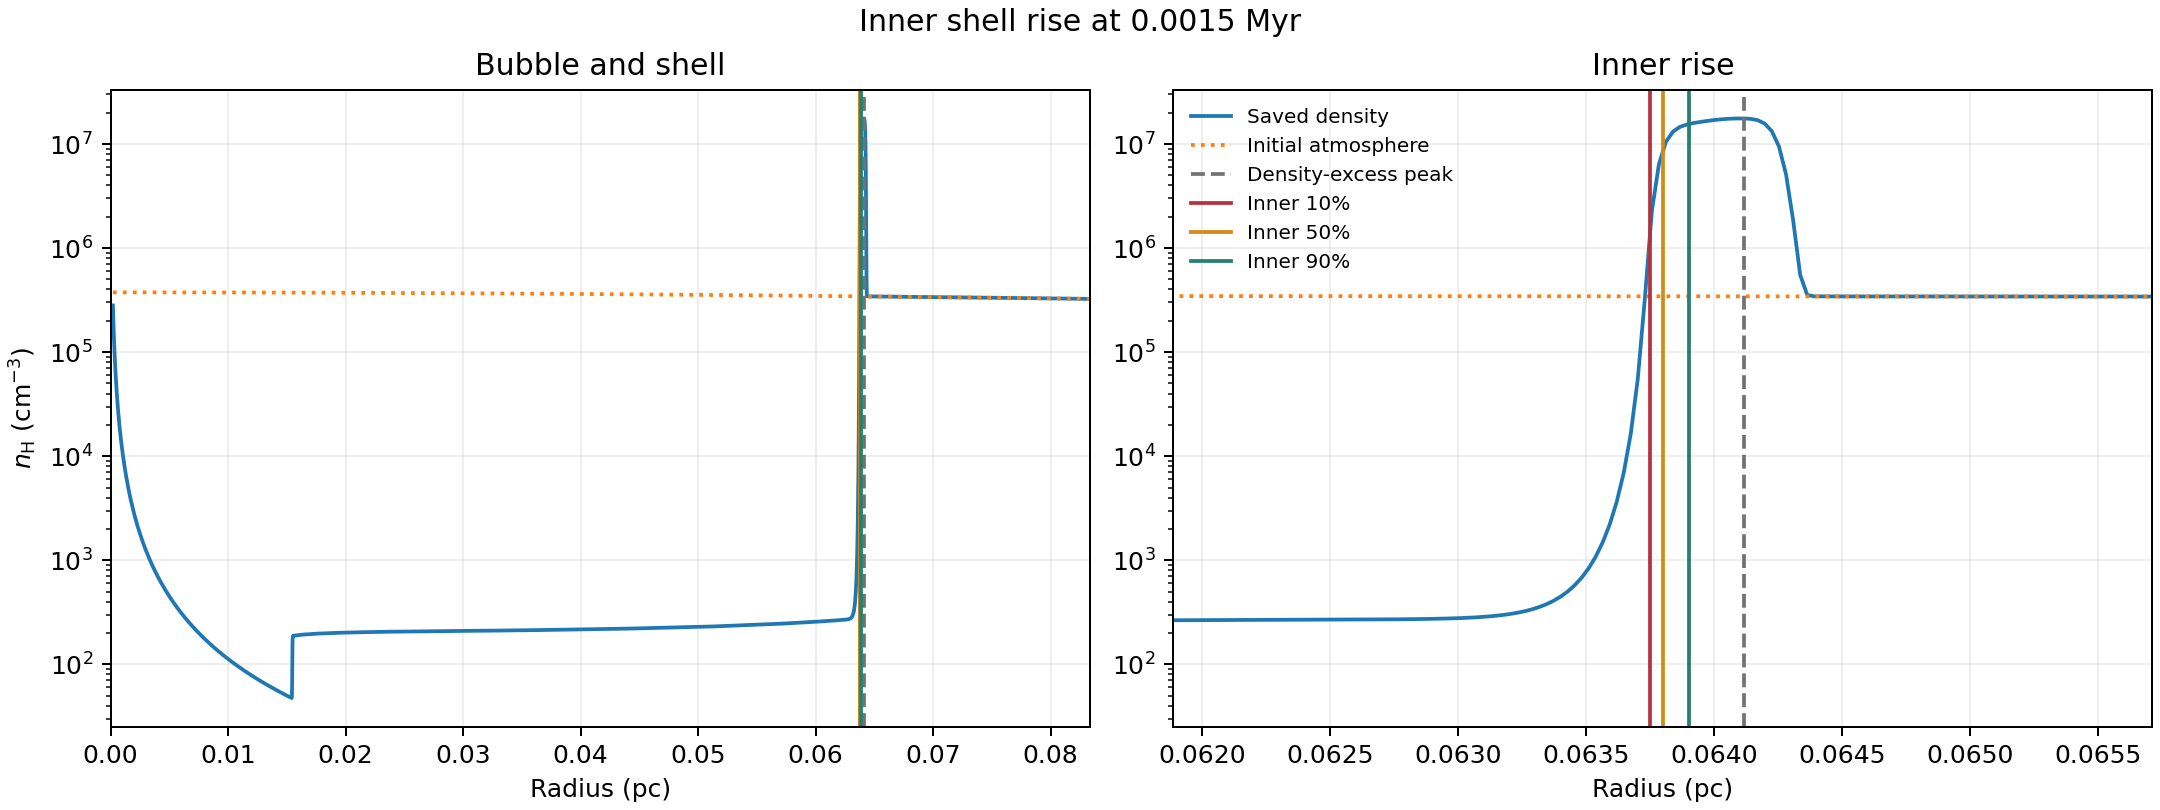
\includegraphics[width=0.98\textwidth,height=0.60\textheight,keepaspectratio]{images/gmc2000_inner_16384.png}
\caption{Validated GMC 2,000 fine-control profile at the same 0.0015-Myr age. The same 2.5-pc evolved boundary and 20-pc atmosphere anchor are used. Both the broad precursor and the local inner rise must remain visible when comparing the new rung.}
\end{figure}

The fine GMC 1,000 and 2,000 runs differ in $R_{10}$ by only 0.000034 pc at this age, much less than either run's change under mesh grading. That observation does not remove uncertainties from direct-WR initial conditions, missing cooling/conduction, the fixed support/gravity model, or the numerical shock width.

\clearpage
\section{New Controlled GMC 1,000 Refinement}
\begin{figure}[htbp]\centering
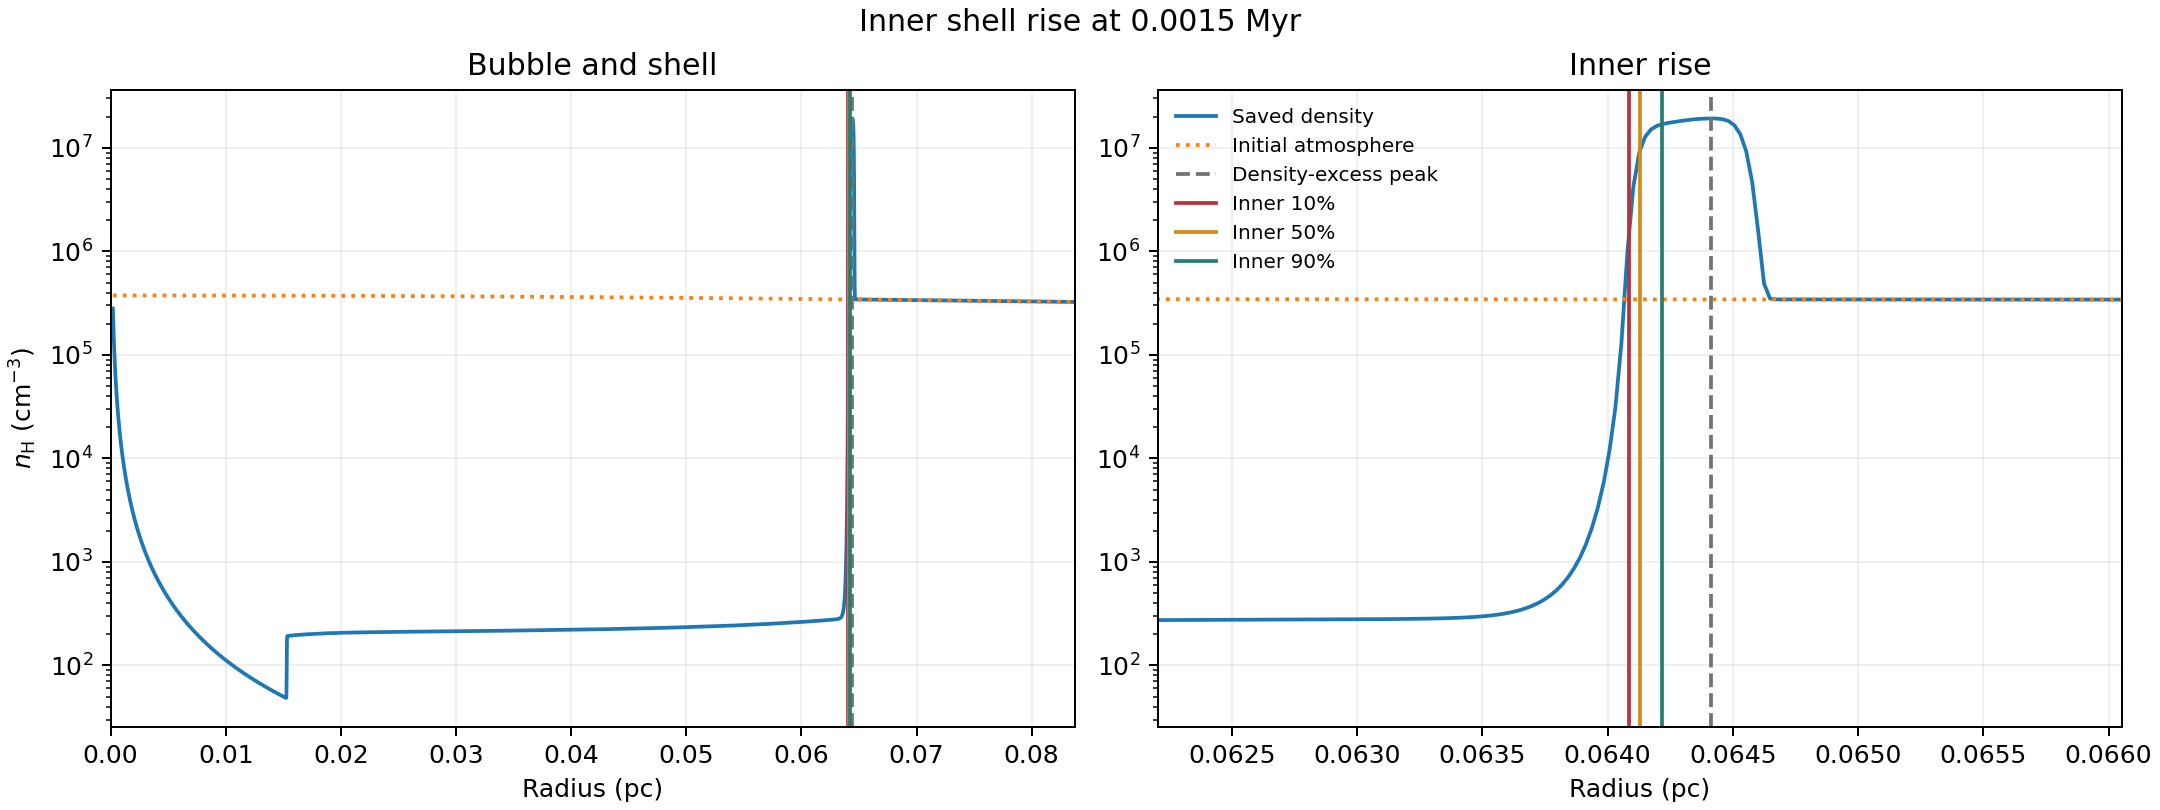
\includegraphics[width=0.98\textwidth,height=0.59\textheight,keepaspectratio]{images/gmc1000_inner_20480.png}
\caption{Independently validated 20,480-cell GMC 1,000 profile at the same 0.0015-Myr age. The left panel retains the whole inward precursor; the right isolates the local inner 10/50/90\% rise. Its $R_{10}=0.064087$ pc and 5.58-cell local rise pass the numerical gates, but the physical rise width has not settled under this controlled mesh change.}
\end{figure}

The endpoint shell has FWHM 17.66 native cells, contrast 55.93, and FWHM/radius 0.0065; its local rise is $1.32\times10^{-4}$ pc. The earlier saved stages include a broad precursor, so this endpoint cannot by itself establish the whole shell trajectory or a WR termination-shock radius. The GMC 2,000 20,480-cell wind has \emph{not} run: only its static control is validated.

\clearpage
\section{Radius Coverage and Fit Context}
\begin{figure}[htbp]\centering
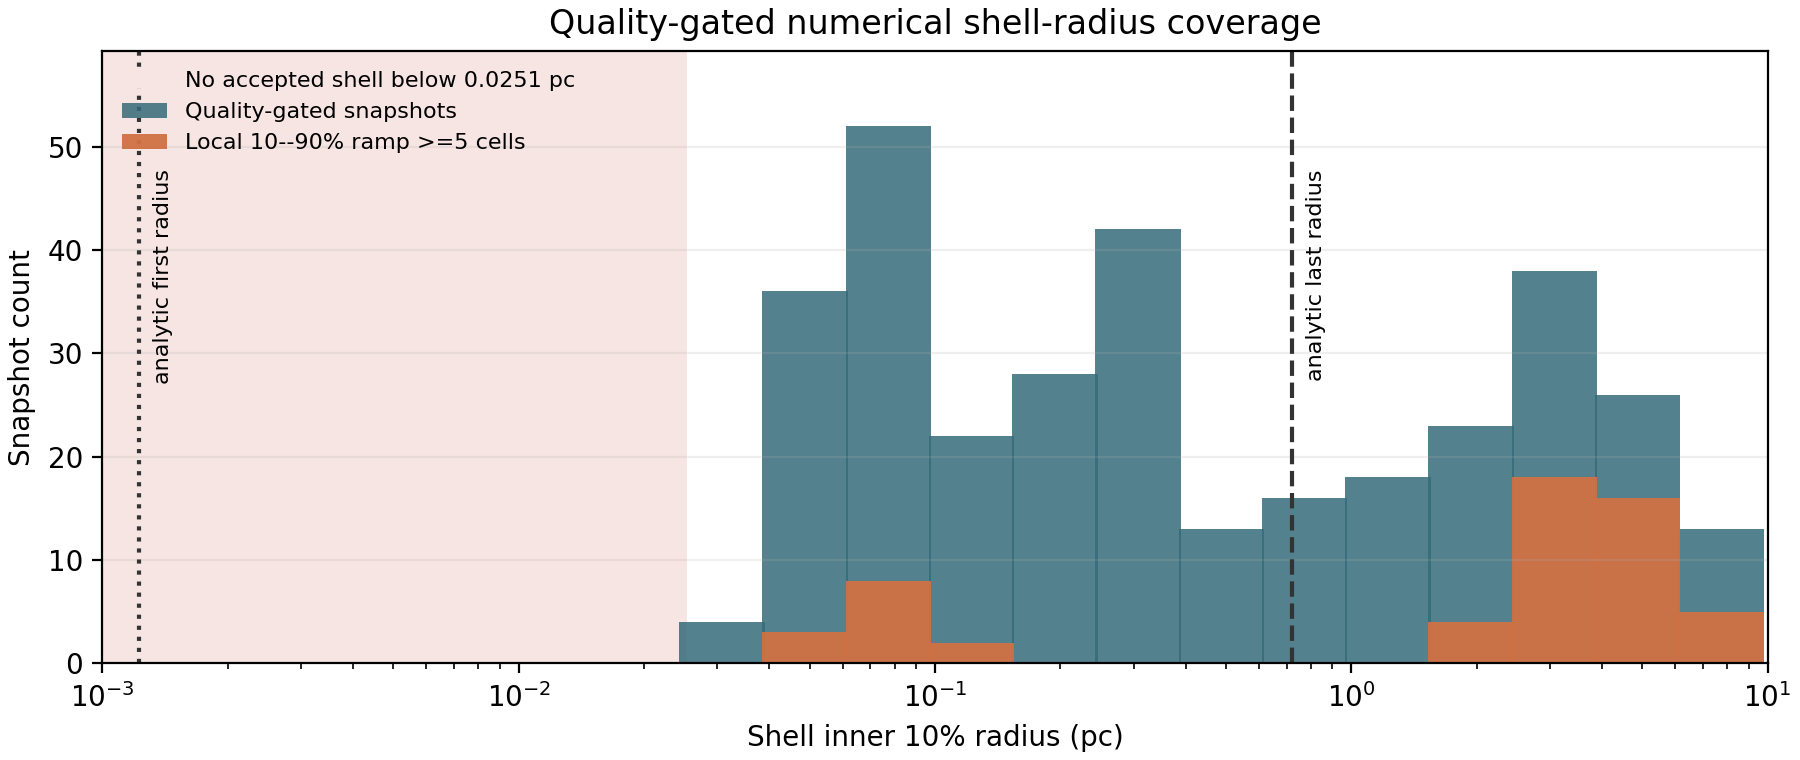
\includegraphics[width=0.98\textwidth,height=0.54\textheight,keepaspectratio]{images/coverage_v28.png}
\caption{Inventory v28, using only snapshots passing the numerical shell gate. Orange counts have an additional five-cell local-rise criterion. Vertical lines mark the selected analytic first/last GRB radii only for scale; they are not measured bubble walls or a forced fit.}
\end{figure}

\begingroup\small\renewcommand{\arraystretch}{1.06}
\begin{tabularx}{\textwidth}{@{}p{0.32\textwidth}rr>{\raggedright\arraybackslash}X@{}}
\toprule
Radius interval (pc) & Accepted & Resolved rise & Interpretation \\
\midrule
0.0010--0.0251 & 0 & 0 & The most inward GRB-scale radii remain untested by a quality-gated shell. \\
0.0251--0.0398 & 4 & 0 & Four accepted snapshots; no five-cell local rise. \\
0.0398--0.0631 & 36 & 3 & Three snapshots have a resolved local rise. \\
Full 0.001--10 range & 331 & 56 & Thirteen of twenty log bins are occupied; counts are snapshots, not independent models. \\
\bottomrule
\end{tabularx}
\endgroup

\clearpage
\section{Controlled 20,480-Cell Rung: One Wind Validated}
The next rung holds the first native width at $1.25\times10^{-5}$ pc, the inner boundary at 0.0002 pc, the 2.5/20-pc evolved/atmosphere radii, and all physical parameters fixed. Only \texttt{domain\_nx1} changes from 16,384 to 20,480 and the required \texttt{qstretch\_baselevel} changes from 1.0002367446884142 to 1.0001749835610765. This modestly refines the shell region without changing the cloud or wind model.

\begingroup\small\renewcommand{\arraystretch}{1.08}
\begin{tabularx}{\textwidth}{@{}>{\raggedright\arraybackslash}p{0.16\textwidth}>{\raggedright\arraybackslash}p{0.28\textwidth}>{\raggedright\arraybackslash}X@{}}
\toprule
Case & No-wind control & WR stage \\
\midrule
GMC 1,000 & Passed independent validation; 33,576-s AMRVAC runtime on Pauley404-02. & Passed guard exit 0, one finish marker, empty stderr, seven VTUs, exact age, WR speed/flux and outer-state validation in 27,204 s. Numerical shell and local-rise gates pass at 0.0015 Myr. \\
GMC 2,000 & Passed independent validation; 60,722-s AMRVAC runtime on Pauley404-03, with guard exit 0, one marker, empty stderr and two VTUs. & Not launched. Host-measured scaling projects 49,375 s, above the 34,560-s safety ceiling (80\% of the 43,200-s guard). Held for a postmeeting guard decision; no automatic change. \\
\bottomrule
\end{tabularx}
\endgroup

Mac03's first system-Python dispatch stopped before AMRVAC because of its existing Xcode license state. Its active static uses Homebrew Python; the failed dispatch log is preserved and no Xcode setting was changed.

\textbf{Decision test at the meeting.} The validated GMC 1,000 refinement makes a matched-age radius/width comparison possible, but a single new rung is not convergence. Jonathan has paused all new long launches until the meeting. The GMC 2,000 matching wind remains held even afterward unless its guard and margin are separately reconsidered; its static success alone is not a GMC 2,000 shell result. No identical-input retry or physics change is authorized.

\section{Reproducibility and Limits}
The companion \texttt{PROVENANCE.md} gives exact manifests, validated result trees, figure sources, SHA-256 pins, and the held stage. The book is built from validated, non-overwriting result and diagnostic trees. The coverage plot reads the v28 quality-gated CSV, not an unvalidated run directory. This pilot does not simulate the full 4.77-Myr stellar history or an MS/RSG-preconditioned WR bubble; it does not establish a physical shock width, convergence, a GRB wall, or agreement with any selected negative-$k$ fit. Cooling, conduction, fixed-gravity, and support changes are separate physics decisions.

\end{document}
